\documentclass[a4paper, 12pt]{report}

% Packages
\usepackage[protrusion=false]{microtype}
\usepackage{setspace}

% Language Package
\usepackage[hidelinks]{hyperref}
\usepackage[italian]{babel}
\usepackage[italian]{cleveref}
\usepackage[toc,page]{appendix}
\usepackage{graphicx}
\usepackage[font=footnotesize,labelfont=bf]{caption}

% Environments
\newenvironment{packed_enum}{
\begin{enumerate}
        \setlength{\itemsep}{1pt}
        \setlength{\parskip}{0pt}
        \setlength{\parsep}{0pt}
}{\end{enumerate}}

\newenvironment{packed_itemize}{
\begin{itemize}
        \setlength{\itemsep}{1pt}
        \setlength{\parskip}{0pt}
        \setlength{\parsep}{0pt}
}{\end{itemize}}

% Initialization
\title{Relazione Progetto HPC 2023}
\author{Michele Montesi \\
        Matricola: 0000974934 \\
        E-Mail: michele.montesi3@studio.unibo.it}

\date{\today}

\begin{document}
\maketitle
% \tableofcontents

\chapter*{Introduzione}
\begin{sloppypar}
La presente ricerca presenta lo sviluppo di due versioni parallelizzate del software \texttt{sph.c}, 
implementate utilizzando la libreria \texttt{OpenMP} e la libreria \texttt{MPI} rispettivamente. 
L'obiettivo della ricerca è quello di valutare i vantaggi prodotti dall'utilizzo della programmazione multi-processore.
\end{sloppypar}

\bigskip

\begin{sloppypar}
\noindent
Per valutare le prestazioni del software, è stato creato uno script in linguaggio Python che esegue il programma 
con un numero crescente di thread, partendo da 1 e arrivando a 12, e con un numero di particelle che varia da 1400 
a 5700. Lo script registra i dati rilevanti in un foglio di lavoro Excel, dai quali verrà calcolata la media.
Queste informazioni saranno poi utilizzate per valutare le prestazioni.

\bigskip
\noindent
I software sono sati testati sul server \texttt{ISI-Raptor}

\end{sloppypar}

{\let\clearpage\relax\chapter*{Versione OpenMP}}
\section*{Implementazione}
\begin{sloppypar}
  \noindent
  In questa implementazione del software, effettuata con \textit{OpenMP}, sono state parallelizzate le sezioni di codice
  che richiedono maggiore elaborazione utilizzando la direttiva \texttt{\#pragma omp parallel for}.

  \smallskip
  \noindent
  Dove necessario sono state effetuate riduzioni al fine di ottimizzare le prestazioni del software parallelizzato.
\end{sloppypar}

\section*{Prestazioni}
\begin{sloppypar}
  \noindent
  Dalla figura \ref{fig:omp_speedup} si nota come all'aumentare del numero di thread, lo \textit{speedup} aumenti in modo significativo,
  come si può notare dall'aumento della curva. Tuttavia, dopo aver raggiunto 8 thread, si può notare una fase di 
  saturazione, in cui l'aumento del numero di thread non porta più 
  a un miglioramento significativo delle prestazioni. In questo punto, l'utilizzo di thread aggiuntivi potrebbe 
  peggiorare le prestazioni. 

  \begin{figure}[ht]
    \centering
    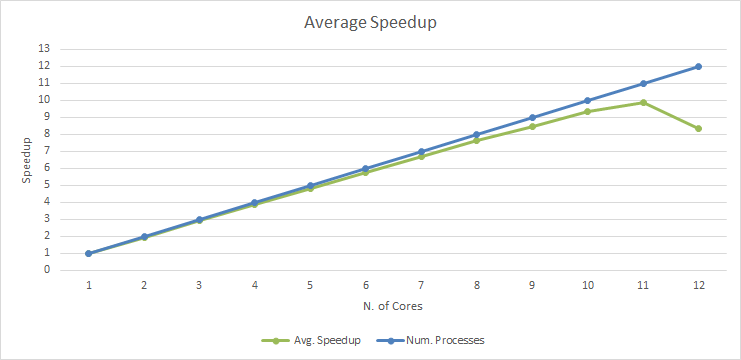
\includegraphics[width=9cm]{img/omp-speedup.png}
    \caption{OpenMP implementation's average speedup}
    \label{fig:omp_speedup}
  \end{figure}

  \noindent
  Dal grafico in figura \ref{fig:omp_sse} si può notare come la \textit{Strong Scaling Efficiency} raggiunga
  il suo picco massimo per circa 6 thread, corrispondente a un'efficienza di circa il 90\% rispetto 
  all'efficienza ideale. Dopo il picco, questa inizia a diminuire, il che significa 
  che l'aggiunta di thread aggiuntivi non porta a un miglioramento significativo delle prestazioni, 
  e può addirittura causare un degrado delle prestazioni complessive.

  \begin{figure}[ht]
    \centering
    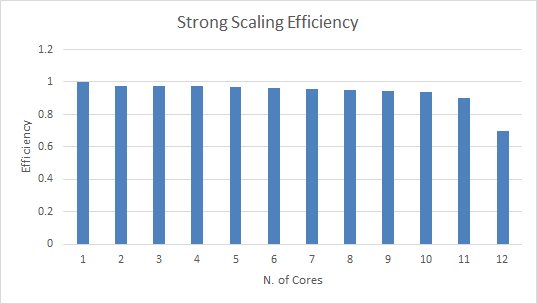
\includegraphics[width=9cm]{img/omp-sse.png}
    \caption{OpenMP implementation's average strong scaling efficiency}
    \label{fig:omp_sse}
  \end{figure}

  \bigskip
  \noindent
  Nella figura \ref{fig:omp_wse} si può notare come la \textit{Weak Scaling Efficiency} rimanga costante 
  all'aumentare della dimensione del problema. Questo indica che il software è in grado di gestire in 
  modo efficiente problemi di dimensioni diverse, distribuendo il carico di lavoro tra le CPU disponibili 
  senza una diminuzione significativa delle prestazioni. Questa costante è un'indicatore
  di una buona scalabilità del software. A 12 thread, l'efficienza debole cala, indicando che l'aggiunta diulteriori CPU
  non comporta migliori prestazioni.



  \begin{figure}[ht]
    \centering
    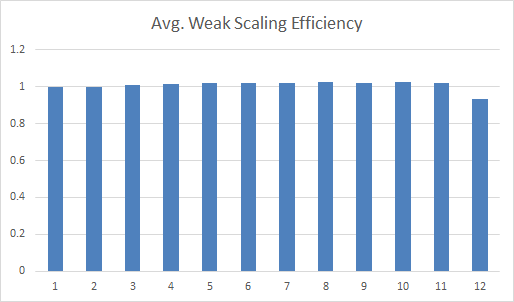
\includegraphics[width=9cm]{img/omp-wse.png}
    \caption{OpenMP implementation's average weak scaling efficiency}
    \label{fig:omp_wse}
  \end{figure}
\end{sloppypar}

{\let\clearpage\relax\chapter*{Versione MPI}}
\section*{Implementazione}
Per l'implementazione del software con \texttt{MPI} è stato creato un \texttt{MPI\_Datatype} contiguo per incapsulare la struttura
dati durante lo scambio di messagi. Per suddividere le particelle fra tutti i processori viene fatta una \texttt{MPI\_Scatterv} dal processo 0.
Dopo \texttt{compute\_density\_pressure} e \texttt{integrate} viene chiamata una \texttt{MPI\_Allgatherv} per raccogliere i dati elaborati
e ridistribuirli nuovamente a tutti i processori mentre per \texttt{compute\_forces} non viene fatto in quanto questo agisce solamente in locale.
Alla fine, dopo aver calcolato la velocità media delle particelle locali, viene eseguita una \texttt{MPI\_Reduce} con operatore somma.
Questo risultato viene diviso per tutti i processi ottenendo così la velocità media complessiva.

\section*{Prestazioni}


\chapter*{Conclusioni}

\end{document}